\begin{figure}[h!]
	\centering
	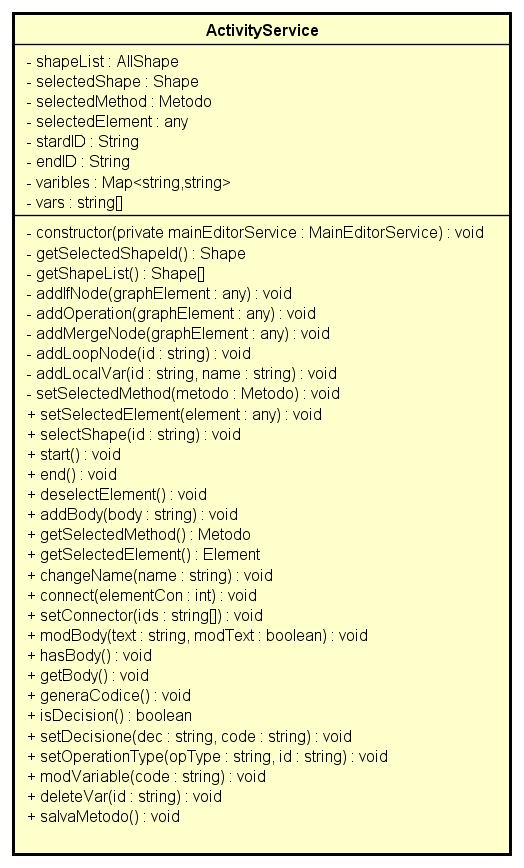
\includegraphics[scale=0.8]{res/sections/SpecificaFrontEnd/Services/Disegnetti/activity.png}
	\caption{Diagramma della classe ActivityService}
\end{figure}

\begin{itemize}
	\item \textbf{Descrizione:}\\
	Servizio che permette la realizzazione di diagrammi di attività, permettendo l'aggiunta e modifica degli shape previsti, e le relative connessione.
	\item \textbf{Utilizzo:}\\
	É possibile realizzate diagrammi di sequenza con le relative shape.
	
	\item \textbf{Attributi:}
		\begin{itemize}
			\item \emph{-shapeList:AllShape}\\
			Lista della shape
			\item \emph{-selectedShape: Shape}\\
			Shape selezionata
			\item \emph{-selectedMethod: Metodo}\\
			Metodo selezionato
			\item \emph{-selectedElement: any}\\
			Elemento selezionato
			\item \emph{-stardID: string}\\
			Id dell'elemento start
			\item \emph{-endID: string}\\
			Id dell'elemento end
			\item \emph{-varibles: Map<string, string>}\\
			Lista dei parametri
			\item \emph{-vars: string[]}\\
			Lista delle variabili
		\end{itemize}
	\item \textbf{Metodi:}
		\begin{itemize}
			\item \emph{-constructor(private mainEditorService: MainEditorService}\\
    		Costruttore della classe\\
    		\textbf{Parametri:}
    		\begin{itemize}
    			\item \emph{mainEditorService: MainEditorService}\\
    			Crea un istanziazione di MainEditorService
    		\end{itemize}
    		\item \emph{-getSelectedShapeId()}\\
    		Ritorna l'id della shape selezionata
    		\item \emph{-getShapeList()}\\
    		Ritorna la lista della shapes
    		\item \emph{-addIfNode(graphElement: any)}\\
    		Aggiunge un if statement\\
    		\textbf{Parametri:}
    		\begin{itemize}
    			\item \emph{graphElement: any}\\
    			Si riferisce al diagramma
    		\end{itemize}
    		\item \emph{-addOperation(graphElement: any)}\\
    		Aggiunge un operazione\\
    		\textbf{Parametri:}
    		\begin{itemize}
    			\item \emph{graphElement: any}\\
    			Si riferisce al diagramma
    		\end{itemize}
    		\item \emph{-addMergeNode(graphElement: any)}\\
    		Aggiunge un merge\\
    		\textbf{Parametri:}
    		\begin{itemize}
    			\item \emph{graphElement: any}\\
    			Si riferisce al diagramma
    		\end{itemize}
    		\item \emph{-addLoopNode(id: string)}\\
    		Aggiunge un ciclo\\
    		\textbf{Parametri:}
    		\begin{itemize}
    			\item \emph{id: string}\\
    			Id della shape
    		\end{itemize}
    		\item \emph{-addLocalVar(id: string, name: string)}\\
    		Aggiunge una variabile locale\\
    		\textbf{Parametri:}
    		\begin{itemize}
    			\item \emph{id: string}\\
    			Id della shape
    			\item \emph{name: string}\\
    			Nome della variabile
    		\end{itemize}
    		\item \emph{-setSelectedMethod(metodo: Metodo)}\\
    		Setta il metodo selezionato\\
    		\textbf{Parametri:}
    		\begin{itemize}
    			\item \emph{metodo: Metodo}\\
    			Metodo da selezionare
    		\end{itemize}
    		\item \emph{+setSelectedElement(element: any)}\\
    		Setta l'elemento selezionato\\
    		\textbf{Parametri:}
    		\begin{itemize}
    			\item \emph{element: any}\\
    			Elemento selezionato
    		\end{itemize}
    		\item \emph{+selectShape(id: string)}\\
    		Seleziona la shape\\
    		\textbf{Parametri:}
    		\begin{itemize}
    			\item \emph{id: string}\\
    			Id della shape da seleionare
    		\end{itemize}
    		\item \emph{+start()}\\
    		Permette di aggiunger una shape start
    		\item \emph{+end()}\\
    		Permette di aggiungere una shape end
    		\item \emph{+deselectElement()}\\
    		Deseleziona l'elemento
    		\item \emph{+addBody(body: string)}\\
    		Aggiunge il body della shape\\
    		\textbf{Parametri:}
    		\begin{itemize}
    			\item \emph{body: string}\\
    			Body della shape
    		\end{itemize}
    		\item \emph{+getSelectedMethod()}\\
    		Ritorna il metodo selezionato
    		\item \emph{+getSelectedElement()}\\
    		Ritorna l'elemento selezionato
    		\item \emph{+getNameMethod()}\\
    		Ritorna il nome del metodo
    		\item \emph{+getVarVis()}\\
    		Ritorna il valore di vars
    		\item \emph{+getShapeType()}\\
    		Ritorna il tipo della shape
    		\item \emph{+changeName(name:string)}\\
    		Modifica il nome della shape\\
    		\textbf{Parametri:}
    		\begin{itemize}
    			\item \emph{name: string}\\
    			Nuovo nome della shape
    		\end{itemize}
    		\item \emph{+connect(elementCon: any)}\\
    		Linka la shape\\
    		\textbf{Parametri:}
    		\begin{itemize}
    			\item \emph{elementCon: any}\\
    			Shape da linkare
    		\end{itemize}
    		\item \emph{+setConnector(ids: string[])}\\
    		Connette la shape\\
    		\textbf{Parametri:}
    		\begin{itemize}
    			\item \emph{ids: string[]}\\
    			Id della shape da connettere
    		\end{itemize}
    		\item \emph{+modBody(text: string, modText: boolean)}\\
    		Modifica il body della shape\\
    		\textbf{Parametri:}
    		\begin{itemize}
    			\item \emph{text: string}\\
    			Nuovo valore
    			\item \emph{modText: boolean}\\
    			Nuovo valore
    		\end{itemize}
    		\item \emph{+hasBody()}\\
    		Controlla se ha un body
    		\item \emph{+getBody()}\\
    		Restituisce il body
    		\item \emph{+generaCodice()}\\
    		Genera il codice
    		\item \emph{+isDecision()}\\
    		True se è una decisione
    		\item \emph{+isVarDeclaration()}\\
    		True se è una dichiarazione
    		\item \emph{+setDecisione(dec: string, code: string)}\\
    		Setta il nuovo valore della decisione\\
    		\textbf{Parametri:}
    		\begin{itemize}
    			\item \emph{dec: string}\\
    			Nuovo valore
    			\item \emph{code: string}\\
    			Codice
    		\end{itemize}
    		\item \emph{+setOperationType(opType: string, id: string)}\\
    		Setta il tipo di operazione\\
    		\textbf{Parametri:}
    		\begin{itemize}
    			\item \emph{opType: string}\\
    			Tipo di operazione
    			\item \emph{id: string}\\
    			Id della shape
    		\end{itemize}
    		\item \emph{+modVariable(code: string)}\\
    		Setta il nuovo valore della variabile\\
    		\textbf{Parametri:}
    		\begin{itemize}
    			\item \emph{code: string}\\
    			Nuovo valore
    		\end{itemize}
    		\item \emph{+deleteVar(id: string)}\\
    		Elimina una variabile\\
    		\textbf{Parametri:}
    		\begin{itemize}
    			\item \emph{id: string}\\
    			Id della variabile da eliminare
    		\end{itemize}
    		\item \emph{+salvaMetodo()}\\
    		Salva il metodo
		\end{itemize}
\end{itemize}